
\documentclass[a4paper]{article}
\usepackage{pslatex}
\usepackage[T1]{fontenc}
\usepackage[utf8x]{inputenc}
\setlength\parskip{\medskipamount}
\setlength\parindent{0pt}
\usepackage{graphicx}
\usepackage{amssymb}
%\usepackage{hyperref}

\usepackage{multicol}

\makeatletter

\providecommand{\boldsymbol}[1]{\mbox{\boldmath $#1$}}
\newcommand{\ASL}			{ASL}
\newcommand{\OSC}[1]		{\texttt{#1}}
\newcommand{\lra}			{$\leftrightarrow$}
\newcommand{\seg}[1]		{Seg(#1)}

\setlength{\parskip}{1mm}

\makeatother

\begin{document}

\title{FaustLive - Implementation \\ v.1.2}

\author{Grame, Centre National de Création Musicale\\
{\small <research@grame.fr>} \\
\vspace{2mm}
[ANR-12-CORD- 0009] and [ANR-13-BS02-0008]
}

\maketitle

\topskip0pt

\newpage
\tableofcontents

\newpage
\section{General Considerations}

\subsection{FaustLive}
FaustLive is an advanced self-contained prototyping environment for the Faust programming language with an ultra-short edit-compile-run cycle. Thanks to its fully embedded compilation chain, FaustLive is simple to install and doesn't require any external compiler, development toolchain or SDK to run. FaustLive is the ideal tool for fast prototyping. Faust programs can be compiled and run on the fly by simple drag and drop. They can even be edited and recompiled while running without sound interruption or Jack disconnection. \\
\\
FaustLive is based on QT. Most classes are a reimplementation of QObjects. 
To know more about these base-objects, see QT documentation : http://qt-project.org/doc/qt-5/classes.html

\subsection{Code Structure}

FaustLive is based on three main classes : FLApp, FLWindow and FLSessionManager.

\begin{itemize}
\item FLApp is a reimplementation of QApplication. Its role is to be a communication center between the menus, dialogs, windows, etc. 

\item FLWindow reimplements QMainWindow. Its role is to contain the DSP, its interface(s) and react to the window's menus/actions/...

\item FLSessionManager is a simple QObject. Its role is to be the compilation center and maintain the hierarchy of the current session. 

\end{itemize}

Many of the dialogs and internal structure classes are singletons to share their information with one shared access point. 

%%%%%%%%%%%%%%%%%FAUSTLIVE APP%%%%%%%%%%%%%%%%%%%
\section{FLApp}
 
FLApp reimplements QApplication. For that matter, it contains the main event loop, where all events from the window system and other sources are processed and dispatched. It also handles the application's initialization (some singletons have to be initialized by FLApp) and finalization.

\subsection{Menus}

\subsubsection{Menu Creation}

The menus are handled differently, depending on the platform. \\
On OSX, the menu of the application appears in the system external menu-bar. Depending on the front window, the specific menu will show. \\
On Windows and Linux, each window of the application has its own menu-bar. There is no general menu-bar. That is why, when the last window is closed, the application quits. \\

While some actions are specific to the windows (edit, export, ...), others have to be treated by the application (new, open, ...). The application-related menus and actions have to be created by the application to be connected to its SLOTs. 

So, FLApp contains the following functions, for menu creation :
\begin{itemize}
\item create\_FileMenu() : QMenu* 
\item create\_ExampleMenu() : QMenu*
\item create\_RecentFileMenu() : QMenu*
\item create\_NavigateMenu() : QMenu*
\item create\_HelpMenu() : QMenu*
\end{itemize}

Because a QMenu cannot be shared between multiple windows, a new one has to be created with each window creation. A list of menus is therefore passed to the window's constructor.

\subsubsection{Menu Reactions}

To react to the menu's actions, FLApp implements a number of SLOTs. These slots are connected to a particular action and contain the reaction. Therefore, most functions in FLApp are direct answers to the menus, handling, for example, the recent sessions and files, the navigation menu, etc.

\subsection{Create a FLWindow}

To create a FLWindow, the FLApp has to choose its settings. There are three different ways to get them  :

\begin{itemize}
\item Create new settings
\item Recall existing settings
\item Copy existing settings
\end{itemize}

In case the settings are new, some parameters have to be initialized like the index of the window (smallest not currently used), the position of the window on screen, ...

Once the FLWindow is created, it is initialized with the Faust source.

%%%%%%%%%%%%%%%%%WINDOW%%%%%%%%%%%%%%%%%
\section{FLWindow}

FLWindow reimplements QMainwindow. Its role is to create the environment of the DSP. It manages its graphical interface(s), its audio interface, etc. Moreover, FLWindow manages the menus, tool bar and status bar, wrapping the DSP's QTInterface. 

\subsection{Interface-s}

One FLWindow contains multiple types of interface, some of which are optional. 

\begin{itemize}
\item QTGUI : interface displayed in FLWindow
\item FUI : interface saving the graphical parameters
\item HTTPUI : interface handling the HTTP protocol for remote control
\item OSCUI : interface handling the OSC protocol for remote control 
\end{itemize}

For each type of interface, FLWindow has a set of functions : allocate, buildUserInterface, run, delete. \\

The synchronization between all the interfaces sharing a unique DSP is done in the QTGUI. The problem being that if we don't have this QTGUI (see some use cases described in RemoteFeature.tex), there is no synchronization. For that matter, a class called FLInterfaceManager has been created. It is not yet of a great interest but if those use cases are implemented, it will become essential.

\subsection{Audio client}

The structure of the audio classes is described in section \ref{Audio}.

From the FLWindow point of view, the creation of an audio client is easy. An audioManager is retrieved from the "AudioCreator" and used mostly like any Faust audio, independently from the real audio driver. 

\begin{itemize}
\item init\_audioClient : initializes the audio manager with the client name and the DSP's number of input and output.
\item setDSP : second step of the audio initialization, by passing the DSP to the audio Manager
\item audioShutDown : callback given to the audio manager. In case the audio driver is shut or stops, the FLWindow can take actions. 
\item start/stop\_Audio : self explanatory

\end{itemize}
\subsection{ToolBar}

The class "FLToolBar" shapes the settings of the FLWindow. Whenever a change in the settings is applied, the toolbar reacts by emitting signals. So that from the FLWindow, we have this set of functions :

\begin{itemize}
\item set\_ToolBar : the toolbar has to be created and its signals connected to the window SLOTs
\item resizingSmall/Big : close/open toolbar
\item setWindowsOptions : the options contained in FLToolBar can be modified outside of the toolbar (OSCUI ports for example when already used), so they have to be synchronized
\item modifiedOptions : reaction to the modification of the compilation options from toolbar
\item generateAuxFiles : reaction to the modification of the automatic export options from toolbar
\item switchOsc : enable/disable OSC interface
\item updateOSCInterface : update OSC interface with new port options
\item switchHttp : enable/disable HTTP interface
\item switchRelease : enable/disable factory publication (not yet implemented)
\item switchRemoteControl : enable/disable remote control interface (not yet implemented)
\end{itemize}

\subsection{StatusBar}

The class "FLStatusBar" holds the processing machine parameter and creates the wrapping layout. 

\begin{itemize}
\item set\_StatusBar : the status bar has to be created
\item redirectSwitch : update the window with new machine option
\end{itemize}

\subsection{Menus}

In the constructor, a list of Menus is given to the FLWindow. Moreover, a window-specific menu is added, giving an access point to the following features :

\begin{itemize}
\item edit : opens the file corresponding to the running DSP. If the DSP is not linked to a source file, the user has to save the DSP as a new file.
\item paste : copies the content of the clipboard into the window, activating the update of the window.
\item duplicate : sends a signal, captured by the application, for it to execute the duplication. 
\item view\_qrcode : activates the remote HTTP control and displays the QrCode, corresponding to the HTML interface.
\item view\_svg : opens the corresponding svg-diagram in the default navigator.
\item export\_file : opens the export manager, allowing the user to export its DSP
\item shut : closes the window
\end{itemize}

\subsection{Drag and Drop}

The FLWindow accepts the Drag and Drop of Faust code as .dsp files, strings, urls but also .wav files. It is set up for that in the constructor, through setAccetDrop(true). The related functions are :

\begin{itemize}
\item dragEnterEvent : describes the accepted mime-types (urls and strings) 
\item dropEvent : updates the window with the new Faust content
\end{itemize}

The FLWindow is also set up to accept "reversed" Drag and Drop. The dragged content is whether a file, a string or a url, depending on the original source of the DSP. 

\begin{itemize}
\item pressEvent : activate reversed Drag and Drop action
\item eventFilter : filters the mouse events when left mouse button is pressed.
\end{itemize}

%%%%%%%%%%%%%%%%%SESSION MANAGER%%%%%%%%%%%%%%%%%
\section{FLSessionManager}

FLSessionManager is a singleton.\\
The role of FLSessionManager is to be the link with libfaust and libfaustremote, to compile the DSPs. Moreover, it has the purpose to maintain the hierarchy of the current session and be able to save/recall sessions and snapshots. 

\subsection{Current Session Hierarchy}

The current session is saved in the user home directory and is called .FaustLive-CurrentSession-versionNumber. On Windows, you can configurate an environment variable FAUSTLIVE\_SESSIONDIR to specify an alternative directory name. \\
The content of the session  is composed of : 
\begin{itemize}
\item Settings.ini : file containing the saved settings as described in FLSettings (\ref{FLSettings}).
\item Examples : folder containing a copy of the example files of the Faust distribution
\item Libs : folder containing a copy of the libraries of the Faust distribution
\item Windows : folder containing the window-specific folders FLW-i, containing :
	\begin{itemize}
		\item Settings.ini : the window specific settings as described in FLWinSettings (\ref{FLWinSettings}).
		\item Graphics.rc : file saving the graphical parameters of the last DSP contained in the window
		\item Connections.jc : file saving the last known Jack connections of the window
		\item SHAKey.dsp* : copy of the Faust code of the last DSP contained in the window (in case the original file is deleted or modified outside of FaustLive execution)
	\end{itemize}
\item SHAFolder : folder containing the DSP-specific folders, containing : 
	\begin{itemize}
		\item SHAKey* : LLVM intermediate representation of the DSP, to accelerate compilation when the same DSP is reused.
		\item SHAKey.dsp*: copy of the Faust code corresponding to this SHAKey
		\item SHAKey-svg* : folder containing the svg diagram resources
	\end{itemize}
\end{itemize}

*To establish an injection between a DSP and its saving files, the SHA-1 hash function is used. This SHAKey is calculated from the Faust code before compilation and its compilation options. That way, one code, compiled with different options is always saved. 

\subsection{DSP compilation}

To compile a DSP, there are two steps :
\begin{itemize}
\item create a factory (builds the protoype of a the DSP class)
\item create an instance of the factory (equivalent of a 'new class" in C++)
\end{itemize}

Because FaustLive enables remote processing, the factories and instances it creates can whether be local (llvm\_dsp\_factory / llvm-dsp ) through libfaust or remote (remote\_dsp\_factory / remote-dsp) through libfaustremote. \\

The goal of FLSession Manager is to be the only class that deals with remote\_dsp\_factory, llvm\_dsp\_factory, remote-dsp, llvm-dsp, ...

The classes that will need compilation will only retrieve a pointer to a dsp, without knowing its type. \\

Still, the two steps cannot be united in the same function, because some audio initialization is needed between the two steps (for the remote case where the sample rate and buffer size are needed to create the instance and only available once the factory is created...).

In conclusion, to create a dsp, there are those two functions :
\begin{itemize}
\item createFactory(const QString\& source, QString\& errorMsg, FLWinSettings* settings = NULL) \\ returns QPair<QString, void*> ;
\item createDSP(QPair<QString, void*> factorySetts, const QString\& source, QString\& errorMsg, FLWinSettings* settings = NULL, RemoteDSPErrorCallback error\_callback = NULL, void* error\_callback\_arg = NULL) \\ returns dsp*;
\end{itemize}

\subsubsection{Create A Factory}

The creation of the factory is described on Figure \ref{fig:Step1} and \ref{fig:Step2}. The final compilation is accomplished through libfaust or libfaustremote, depending on the machineName (described in the settings) (see Figure  \ref{fig:Step2}). The factory is created from a file, saved in the current session and named after a SHAKey. \\

The calculation of this key is presented on Figure  \ref{fig:Step1}. In this process, the compilation options are sorted, following a certain pattern, in order to have -vec -sch giving the same key than -sch -vec. Moreover, the source given to createFactory can be a string, a file, a web url or a wav file. The function sourceToFaustContent has the role to transform any kind of source into a compilable faust content. 

\begin{figure}[!h]
\begin{center}
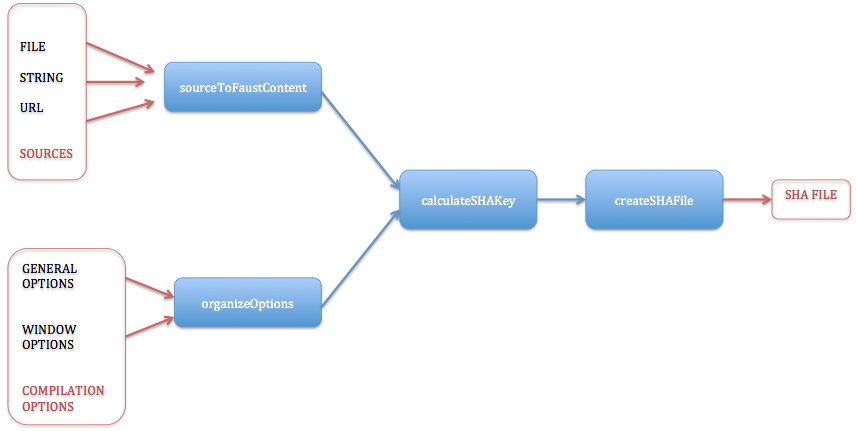
\includegraphics[width=\columnwidth]{images/Step1_Compilation.png}
\caption{Create Factory - Step 1}
\label{fig:Step1}
\vspace{0.5cm}
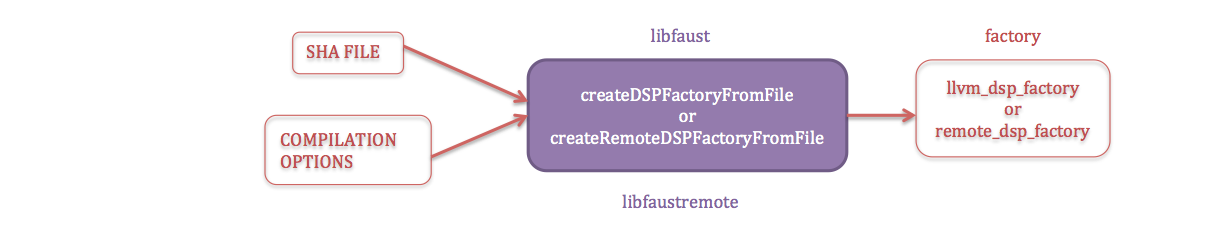
\includegraphics[width=\columnwidth]{images/Step2_Compilation.png}
\caption{Create Factory - Step 2}
\label{fig:Step2}
\end{center}
\end{figure}

\subsubsection{Create An Instance}

This function creates a llvm\_dsp or a remote\_dsp depending on the type of factory passed to the function. Moreover, it saves the new window settings, in case of successfull compilation. The dsp returned is abstract, so that the FLWindow doesn't have the information of real type. 

\subsection{Delete Factories and Instances}

Every DSP created is mapped to its factory, so that when you delete the DSP, FLSessionManager has a track of which factory to delete. 

\subsection{Session/Snapshot Restoration}

When the user recalls a snapshot or opens FaustLive and wishes to have his last session restored, the system has to go through some restoration steps. Those operations have, as goal, to make sure that the resources needed by the session were not deleted or corrupted outside of FaustLive execution. 

\subsubsection{Current Session Restoration}

In case of changes, the user has the choice between : 
\begin{itemize}
\item using the internal copy of the file
\item using the original file and recompile its new content
\end{itemize}

\subsubsection{Recall or Import Snapshots}

In case of snapshot loading, the user is informed that a change was made in his files but the internal copy is always used. This choice was made, considering that when the user has made a snapshot, it is to reload the exact same state, he saved. 

%%%%%%%%%%%%%%%%%NETWORK%%%%%%%%%%%%%%%%%
\section{Network Interactions}

There are different types of remote interfaces, described below. But the logic of them is common. The idea is that each interface is built and runs separately from the FLWindow declaring it. But a central server is used to keep track of all interfaces. That way, a request to that server permits to have a view of all remote interfaces. 

\subsection{HTTP interface}
The HttpUi described in Faust is used to create an Html Interface, synchronized with the local interface. This component embeds a Http server in the application. \\
Moreover, in FaustLive, a central server, called FLServerHttp, handles the Drag and Drop on the remote Html Interface and centralizes the HttpUis. 

Here is the list of request that can be made to the server :\\
http://IPofLocalHost:portConfiguredInPreferences
\begin{itemize}
\item returns the main page of the server, containing only a drop zone for DSP files.
\item {\it /portOfSpecificInterface} : adds the Html page \\(http://IPofLocalHost:portOfSpecificInterface)\\ containing the interface to the main page. By default, the port is 5510. 
\item {\it /portOfSpecificInterface/JSON} : this request is redirected to the interface-specific server (http://IPofLocalHost:portOfSpecificInterface/JSON) and returns the JSON application describing the interface.
\item {\it /availableInterfaces} : returns an html page describing all http interfaces available.
\item {\it /availableInterfaces/Json} : returns the interfaces available as a JSON application.
\end{itemize}

\subsection{OSC interface}

The OSC interfaces are, for now, only used as specific interfaces in the FLWindows. The central OSC server is not yet implemented. 

\subsection{Remote interface}

Not yet implemented. See RemoteFeatures.tex.

%%%%%%%%%%%%%%%%%SETTING STRUCTURE%%%%%%%%%%%%%%%%
\section{Setting Management}

%%%%%%%%%%%%%%%%%GENERAL SETTINGS%%%%%%%%%%%%%%%%%
\subsection{FLSettings \label{FLSettings}}

FLSettings is a singleton. \\ 
It reimplements QSettings. A hierarchy, presented {Figure \ref{fig:FLSettings}, allows us to access the settings easily. \\

The setting file is saved at the root of the current session (/Users/you/.FaustLiveCurrentSession-version).
 
\begin{figure}[!h]
\begin{center}
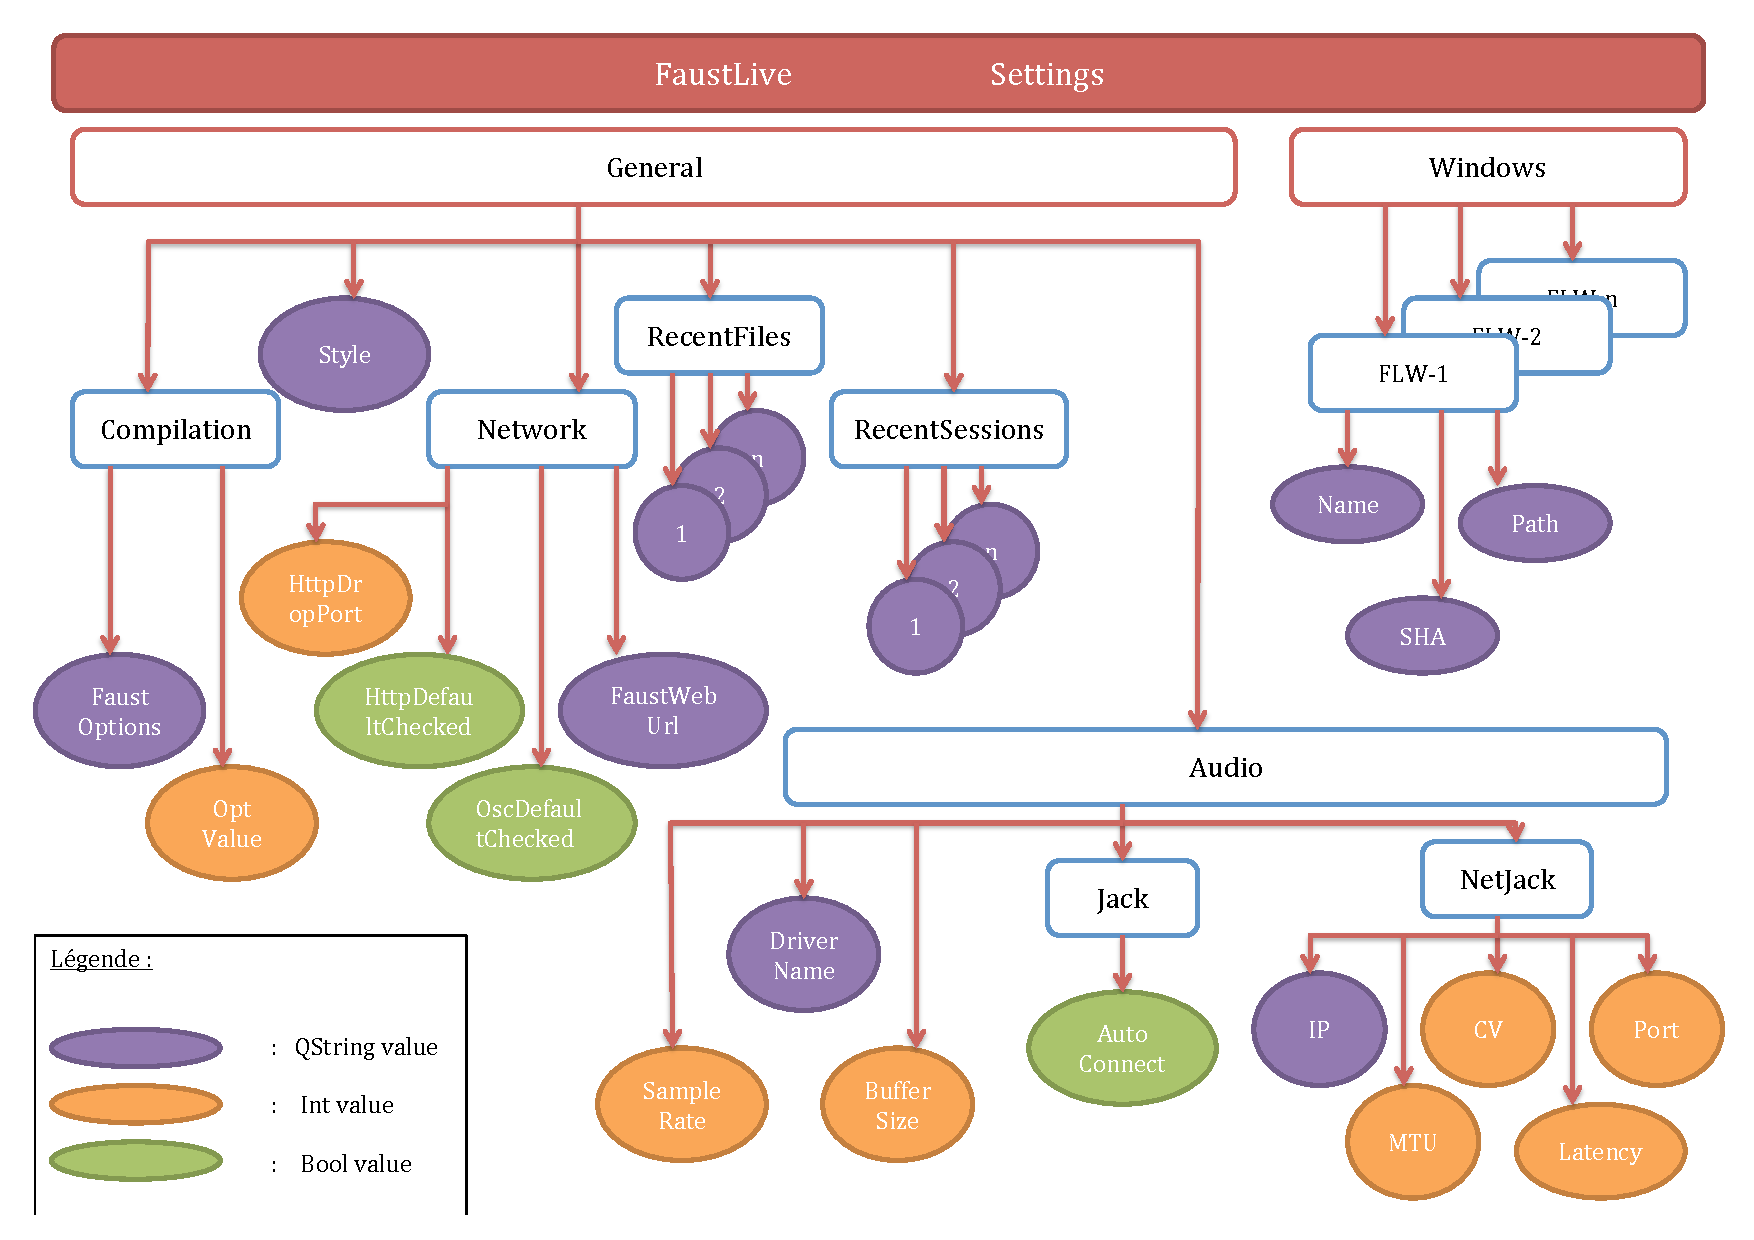
\includegraphics[width=\columnwidth]{images/FLSettings}
\caption{FLSettings structure}
\label{fig:FLSettings}
\end{center}
\end{figure}
 
For example, the value is accessible like this :\\
\textit{int httpPort = FLSettings::\_Instance()->value("General/Network/HttpDropPort", defaultValue);}

%%%%%%%%%%%%%%%%%WINDOW SETTINGS%%%%%%%%%%%%%%%%%
\subsection{FLWinSettings \label{FLWinSettings}}

FLWinSettings reimplements QSettings. But, this class is not a singleton, each FLWindow is associated to a FLWinSettings. 

\begin{figure}[!h]
\begin{center}
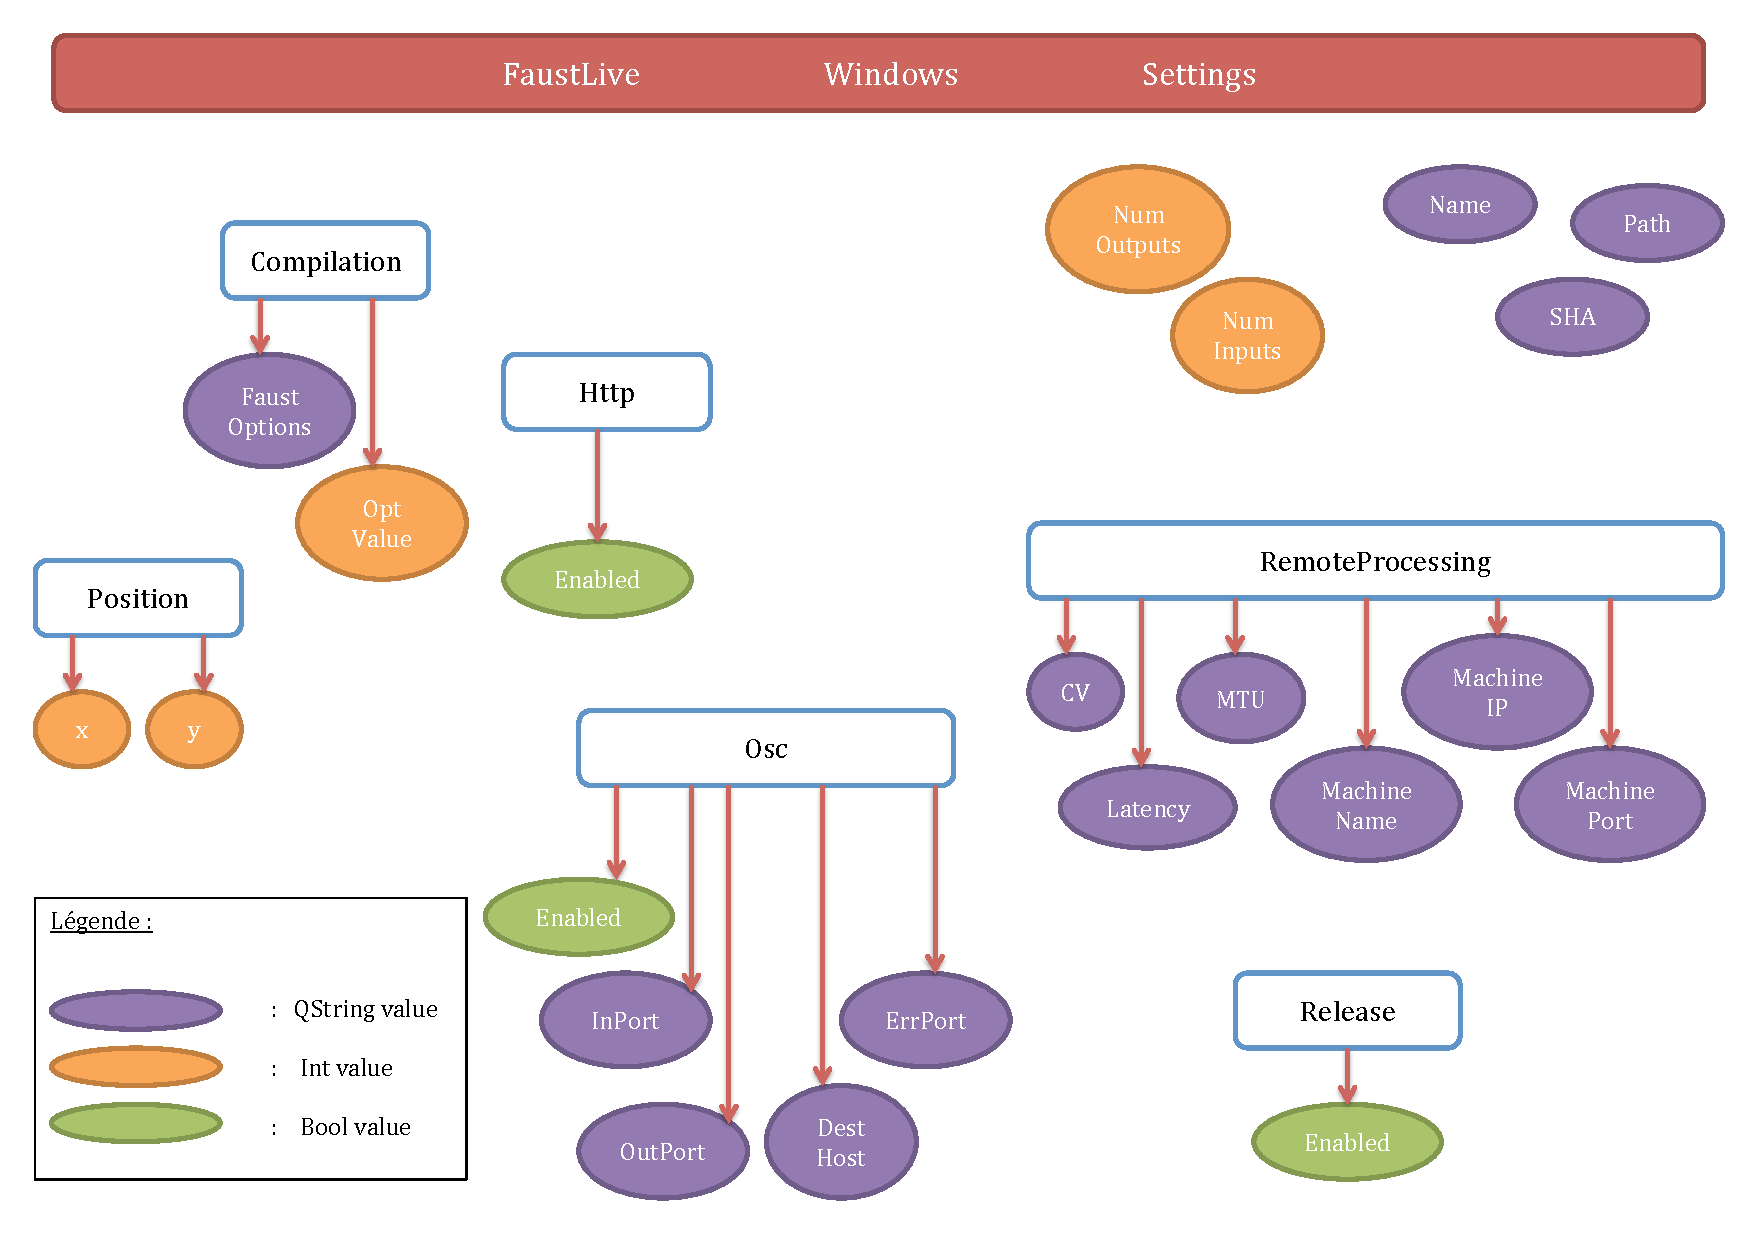
\includegraphics[width=\columnwidth]{images/FLWinSettings}
\caption{FLWinSettings structure}
\label{fig:FLWinSettings}
\end{center}
\end{figure}


For example, the value is accesible like this :\\
\textit{int oscInPort = fSettings->value("Osc/InPort", defaultValue);} \\

The added feature of FLWinSettings, compared to QSettings, is to synchronize three parameters of the window with the general FLSettings. That way, Name, SHA and Path are also accessible from the FLSettings. This feature is really usefull for snaspshot and session restoration, to have a global vision of the existing windows.

%%%%%%%%%%%%%%%%%FILE WATCHER%%%%%%%%%%%%%%%%%
\section{FLFileWatcher}

FLFileWatcher is a singleton. \\
Its role is to maintain the list of files currently used in FaustLive as DSP source or dependency. When a file is modified, renamed or deleted, it is set to redirect the action to the file-corresponding window(s).

Whenever the signal directoryChanged is received on a watched directory, the content is compared to the previous one, in order to know if a file was renamed (same number of children files but new name) or deleted. 

Whenever a watched file is modified in a text editor or another external application, the signal fileChanged is received. The FLWindow is therefore informed that it has to update. 

%%%%%%%%%%%%%%%%%MENUS AND DIALOGS%%%%%%%%%%%%%%%%%
\section{Menus and Dialogs}

Each type of dialog/window used by FaustLive has its own class. It is mostly describing the layout of the dialog and is redirecting the specific actions to the application, connecting the right SLOTs. 

\subsection{FLErrorWindow}

FLErrorWindow reimplements QMainWindow. Its role is to displays all errors occurring in the program.
FLErrorWindow is a singleton.

\subsection{FLMessageWindow}

FLMessageWindow reimplements QDialog. Its role is to displays messages printed by the program, like (Compiling DSP..., etc).
FLMessageWindow is a singleton.

\subsection{FLHelpDialog}

FLHelpDialog reimplements QDialog. Its role is to display the help menu, for the user to get information of FaustLive uses. 

\subsection{FLPreferenceWindow}

FLPreferenceWindow reimplements QMainWindow. Its role is to display the preferences of FaustLive and to handle the changes of settings. 

\subsection{FLPresentationWindow}

FLPresentationWindow reimplements QMainWindow. Its role is to display the presentation menu.

\subsection{FLExportManager}

FLExportManager contains two classes classes describing the two dialogs used in the export process. The first dialog presents all the targets available. The second one shows the progress of the export.

%%%%%%%%%%%%%%%%%AUDIO STRUCTURE%%%%%%%%%%%%%%%%%
\section{Audio \label{Audio}}

In this section, we discuss the way the audio rendering is managed in FaustLive (see also the Appendix).
First, will be described the type of audio driver used into FaustLive and how the linking is done. Then, the algorithm of the crossfade will be explained, taking care of smoothing the transition between two DSPs relaying in the same window. 

\subsection{Audio drivers used by FaustLive}
 
Depending on the operating system and the compiling options, it is possible to embed different audio architectures in FaustLive.
Default drivers are :
\begin{itemize}
\item CoreAudio on OSX
\item JACK on Linux
\item PortAudio on Windows
\end{itemize}

Then JACK, NetJack and PortAudio can be added with make options : JACK=1 NETJACK=1 PORTAUDIO=1.

\subsection{Code Organisation}

The general structure of the code is based on the "abstract factory" pattern. That way, the class "AudioCreator" is the only class knowing which type of driver is used. It is the intermediary between the FLWindow, handling the audio client, and the driver-specific elements.  \\

The abstract factory contains the following pure virtual functions :
\begin{itemize}
\item createAudioSettings(QGroupBox* parent)
\item createAudioManager(AudioShutDownCallaback, void* arg)
\end{itemize}

Then each audio driver has its own set of classes :
\begin{itemize}
\item audioFactory : creates the driver-specific elements through the reimplementation of createAudioSettings and createAudioManager. 
\item audioSettings : contains the settings needed by the driver and their graphical representation (for example a buffer size, a sample rate, ...)
\item audioFader : mixes the audio and crossfade features
\item audioManager : manipulates the audio faders and manages their crossfades 
\end{itemize}

\subsection{Crossfade implementation}

The specification is to smooth the transition between two relaying DSPs in a situation of drag and drop or source edition. If a DSP algorithm is not modified, the transition should not be hearable. \\

Now, to implement this function, some functions are common to all architectures (implement\_crossfade, reset\_crossfade\_values, launch\_crossfade, etc). These features are divided in two classes \footnote{The separation between interface and implementation sometimes had to be made because some audio classes (like coreaudio-dsp) already made the difference (coreaudio/TCoreAudioRenderer). } :
\begin{itemize}
\item AudioFader\_Interface : containing the basic instructions needed by the client to launch a crossfade and know when it stopped. 
\item AudioFader\_Implementation : containing the calculation functions of the crossfade. This class holds the duration of a crossfade, described as a number of audio cycles.
\end{itemize}

The crossfade functions are mixed to the audio features in the driver-specific audioFader classes, by doble inheritance.

\subsection{AudioManager}

The role of the audio manager is to manipulate the audioFader(s) and manage the crossfade. Depending on the driver, there are two approaches of structure :
\begin{itemize}
\item the one managing one audioFader and fading two DSPs in its "process" function (JACK)
\item the one managing two audioFaders, relaying with a fade in for one part and a fade out for the other (CoreAudio, NetJack, PortAudio)
\end{itemize}

\subsection{How to add a new audio architecture}

To add a new type of driver audio in FaustLive, the first step is to implement the driver-specific set of classes :
\begin{itemize}
\item audioFactory
\item audioSettings
\item audioManager
\item audioFader
\end{itemize}

Then, some elements have to be added to the class "AudioCreator" : 
\begin{itemize}
\item add the new architecture to the enum "AudioArchitecture"
\item add a new item in the comboBox "fAudioArchitecture"
\item add a new case in createFactory
\end{itemize}

Finally, FaustLive.pro has to be modified (for each platform compatible with the new driver), in order to add the librairies (through conditional compilation).

%%%%%%%%%%%%%%%%%REMOTE INTERFACES%%%%%%%%%%%%%%%%%
\section{FLComponentWindow}

The component window is a feature allowing the user to compose DSPs in a parallel/sequence/recursive way to create a new DSP. 
As in the FLWindow, it is possible to drop files and urls, so that you can combine elements from the web with local DSPs.

\subsection{Component creation}

The resulting DSP is a sequence of "stereoized parallel DSPs" : DSPs are first composed in parallel, then stereoized (see stereoize in music.lib) and finally put in sequence. The recursive loop is then applied with the function recursivize. \\
Through this process, the resulting DSP is stereo, whatever DSPs were used as components. 

\subsection{Layout optimization}

An "optimized" layout for the resulting DSP is calculated, taking as goal to reduce the surface of the interface. In order to do that, a binary tree of items is created. In this tree there are three types of elements : 
\begin{itemize}
\item leaf nodes : containing the real faust interface
\item vertical containers, putting in a vertical group it's two sub-nodes
\item horizontal containers, putting in a horizontal group it's two sub-nodes. 
\end{itemize}

Each element of the tree has a function render, so that called on the root node, the whole layout is calculated.

%%%%%%%%%%%%%%%%%DISTRIBUTION STRUCTURE%%%%%%%%%%%%%%%%%
\section{Distribution Structure}

FaustLive's distribution has the following hierarchy :
\begin{itemize}
\item Build : Plateform-specific Makefiles and resources
\item Documentation : Faust and FaustLive documentation
\item Resources : examples, libs and all resources needed within FaustLive
\item src : all the sources of FaustLive, structured as :
\begin{itemize}
\item Audio : containing the audio classes, depending on the driver architecture
\item MainStructure : center of FaustLive, containing the three main classes : FLApp, FLWindow and FLSessionManager
\item MenusAndDialogs
\item Network : containing the server(s) embedded in FaustLive (FLHttpServer, coming soon FLOscServer)
\item Utilities
\end{itemize}
\end{itemize}

\subsection{Compile and Install}

Whichever platform you are on, you will have to install some libraries to be able to compile FaustLive :
\begin{itemize}
\item faust / faustremote / httpdfaust 
\item jack2 (unix/windows) or portaudio (windows)
\item libopenssl
\item libmicrohttpd
\item libqrencode
\item libcurl
\item llvm
\item libcrypto
\item liblo
\end{itemize}

You can whether download the packages and compile them yourself or get them through apt-get, macport, brew or some other package installer. 

\subsubsection{Unix}

Once you installed all that, you can execute : \\
{\it cd yourFaustLiveDirectory} \\
{\it make} (JACK=1 NETJACK=1 PORTAUDIO=1 REMOTE=1 depending on the options you want to enable)\\
{\it sudo make install} 

\subsubsection{Windows}

On Windows, you will have to modify FaustLive.pro with your own paths, depending on where you compiled the needed librairies. \\

Then you can execute : \\
{\it qmake -spec win32-msvc2012 (depending on your version of Visual Studio) JVAR=1 NJVAR=1 PAVAR=1 REMVAR=1 (depending on the options you want to enable)} \\
The solution created can be added in a new solution, that you can build and run. 

\subsection{Create a new distribution}

\subsubsection{Unix}

The idea is to create a self-contained application. Therefore, the dependent librairies have to be statically compiled. The following librairies can be easily downloaded and compiled with : 

\begin{multicols}{2}

\begin{itemize}
\item libqrencode
\item libmicrohttpd
\item libcurl
\item libsndfile
\end{itemize}


./configure - -enable-static \\
make \\
sudo make install \\
\end{multicols}

Then, once those libraries are compiled, you can execute {\it make dist} in FaustLive's directory.

\subsubsection{Windows}

To create an installer with FaustLive.exe, you have to install InnoSetup. Then you can modify setup\_file.iss to your needs and run it.

\section{Appendix}

\begin{figure}[!h]
\begin{center}
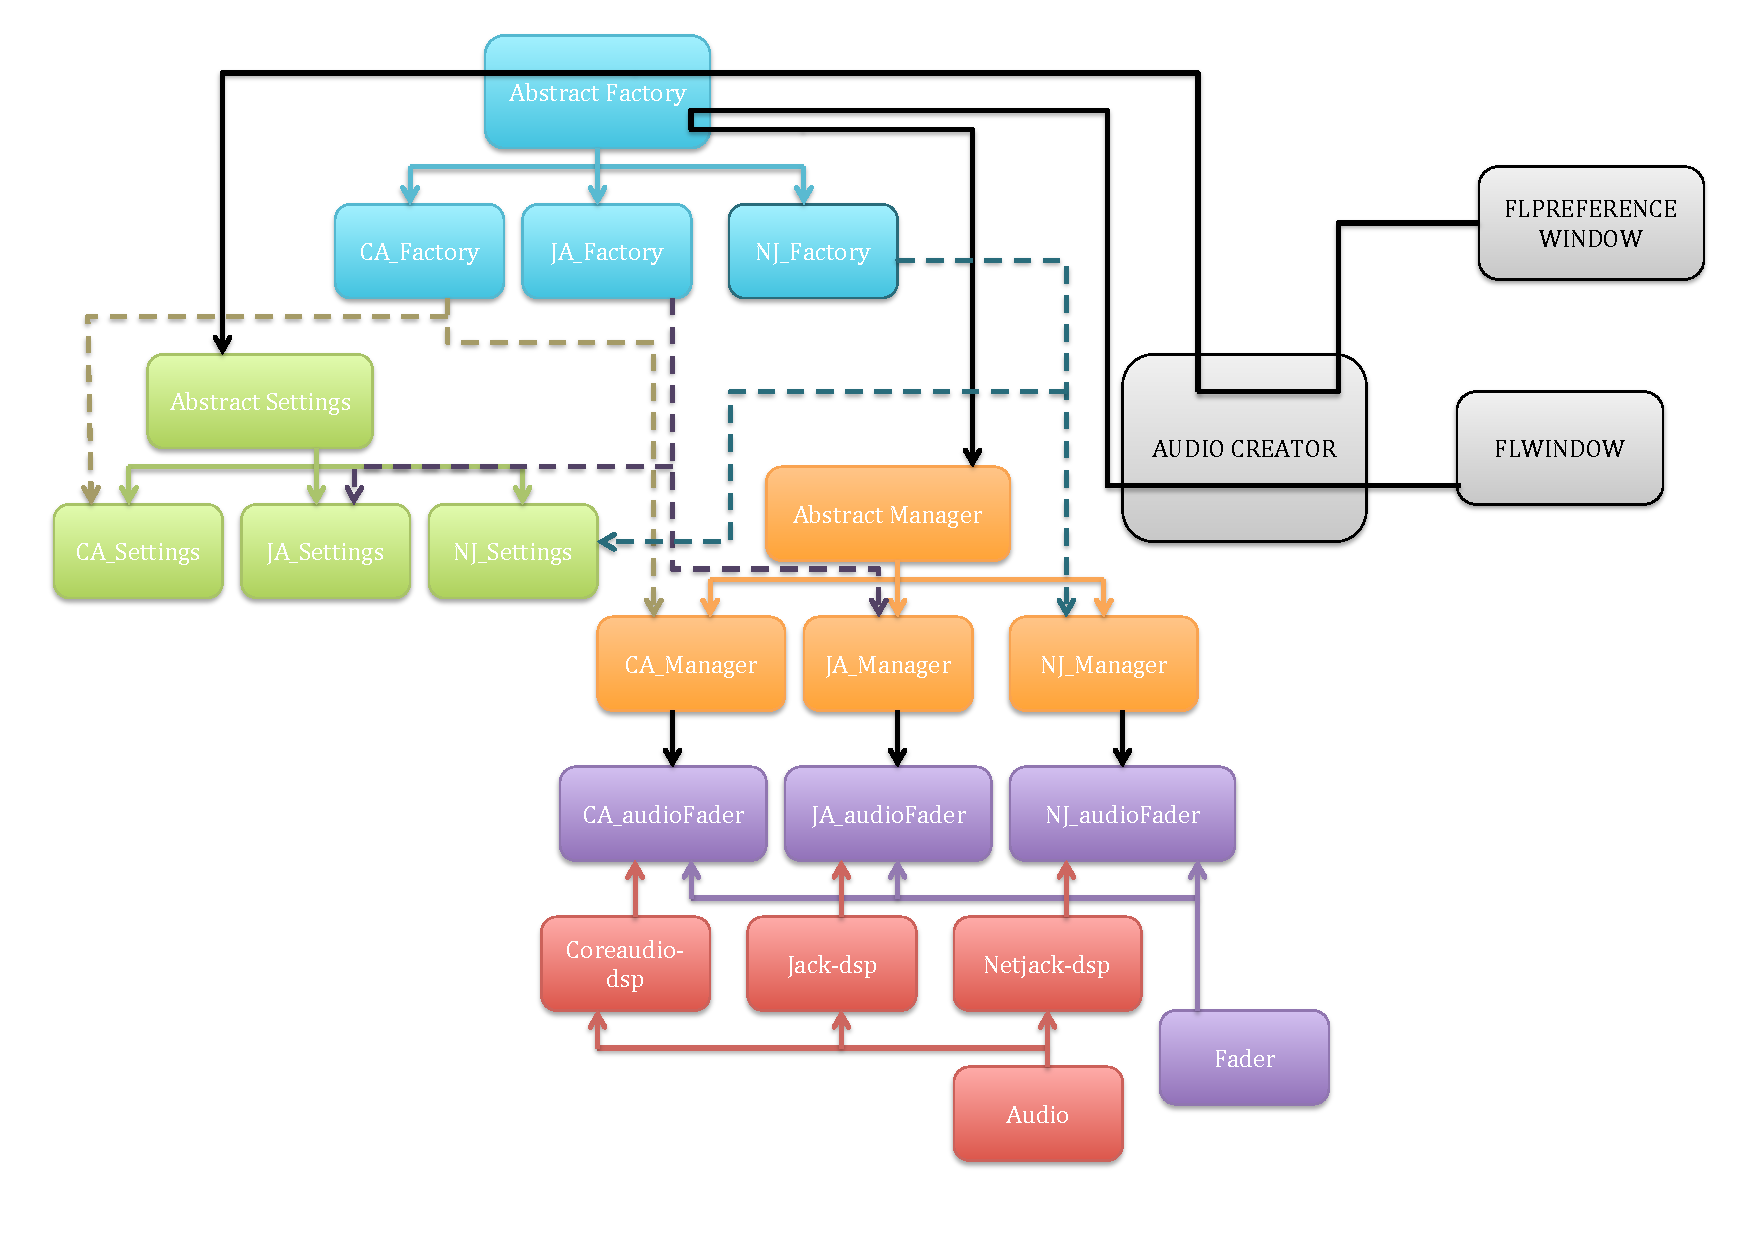
\includegraphics[width=\columnwidth]{images/newAudioStructure}
\caption{Audio Drivers Structure}
\label{fig:FLWinSettings}
\end{center}
\end{figure}

\end{document}




